\section{Analisis Perancangan}
\subsection{Analisis}
Analisis sistem merupakan penguraian dari suatu sistem informasi yang utuh kedalam bagian-bagian komponen dengan tujuan untuk mengidentifikasi dan mengevaluasi permasalahan, kesempatan, hambatan yang terjadi dan kebutuhan yang diharapkan sehingga nantinya dapat diusulkan perbaikannya. Pada bagian ini, akan dibahas tentang analisis prosedur dan aliran dokumen sistem yang sedang berjalan yang digambarkan dalam bentuk flowmap, pengkodean dan analisis sistem non fungsional yang meliputi perangkat keras dan perangkat lunak yang digunakan.
\subsection{Analisis Sistem yang Sedang Berjalan}
Analisis sistem yang sedang berjalan merupakan analisis tahap awal dalam penentuan dan perancangan sistem. Di dalam analisis ini terdapat dua metode yang digunakan, yaitu: analisis prosedur (flowmap) dan analisis dokumen yang digunakan. Dengan demikian, aplikasi yang akan dibangun akan benar-benar sesuai dengan prosedur serta sistem kerja yang dibutuhkan.

\subsection{Analisis Sistem yang Sedang Berjalan pada Absensi Mahasiswa Internship}
Proses pendataan absensi pada mahasiswa internship bisa digambarkan sebagai berikut:
\begin{enumerate}
	\item Pembimbing eksternal di tiap perusahaan internship menyerahkan form absensi ke Mahasiswa
	\item Mahasiswa mengisi form absensi setiap melakukan internship
	\item Mahasiswa menyerahkan form absensi ke pembimbing eksternal perusahaan internship
	\item Jika telah melaksanakan internship, form absensi di cetak dan diserahkan kepada admin program studi masing-masing
\end{enumerate}
	\begin{figure}[H]
		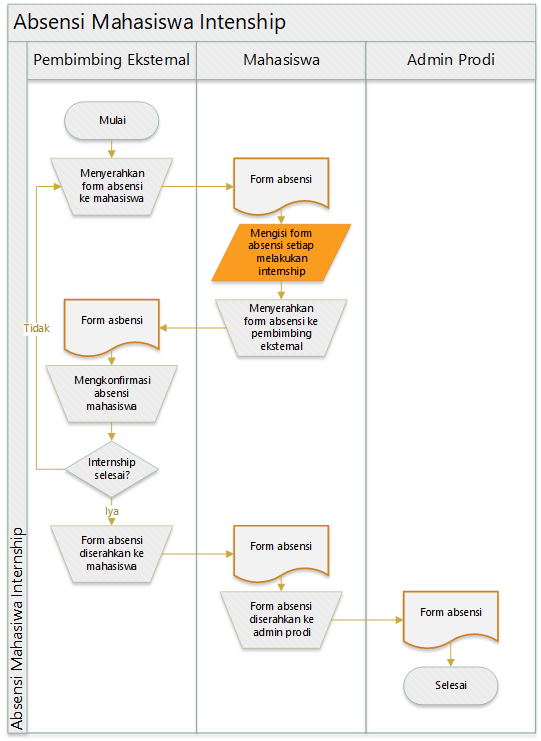
\includegraphics[width=10cm]{figures/image019.png}
		\centering
		\caption{Sistem yang sedang berjalan }
	\end{figure}
\subsection{Analisis Dokumen yang Digunakan}
Dari hasil analisis yang dilakukan, dokumen yang digunakan adalah dokumen absensi mahasiswa internship. Adapun dokumen yang dimaksud adalah sebagai berikut
\begin{table}[h!]
\centering
\begin{tabular}{|c|c|} 
 \hline
 \textbf{Dibuat Oleh}   & Pembimbing Eksternal \\ 
\hline
\textbf{Dibuat Untuk}   & Mahasiswa\\ 
\hline
\textbf{Isi}  & Kegiatan Mahasiswa selama internship\\ 
\hline
\textbf{Frekuensi} & Setiap mahasiswa melakukan internship\\ 
\hline
 \textbf{Tujuan }& Memantau kehadiran dan kegiatan mahasiswa selama internship \\ 
 \hline
\end{tabular}
\caption{Dokumen Absensi Mahasiswa Internship}
\label{table:1}
\end{table}

\subsection{Analisis Sistem yang Akan Dibangun}
Analisis kebutuhan yang dimaksud disini berupa analisis flowmap mengenai sistem yang akan dibangun meliputi proses pendaftaran mahasiswa internship dan absensi mahasiswa internship. Adapun flowmap yang akan dibangun adalah sebagai berikut:
\subsection{Analisis Sistem yang Akan Dibangun Pada Pendaftaran Mahasiswa Internship}
Pada proses pendaftaran mahasiswa internship melibatkan mahasiswa, pembimbing eksternal, pembimbing internal, dan admin prodi. Adapun mekanisme kerja yang dibuat adalah sebagai berikut:
\begin{enumerate}
	\item Mahasiswa mengakses form pendaftaran internship lewat website
	\item Mahasiswa mengisi form pendaftaran internship dan mensubmit datanya
	\item Admin memeriksa data yang disubmit, jika data yang diinputkan benar maka dikirimkan kode QR lewat email
	\item Mahasiswa melakukan registrasi dengan memindai kode QR yang dikirim lewat email lewat aplikasi mobile
	\item Mahasiswa diminta mengisi data perusahaan di lokasi perusahaannya langsung dan mensubmit datanya
	\item Pembimbing Eksternal memeriksa data yang disubmit, jika data yang diinputkan benar maka akan dikonfirmasi mahasiswa yang mendaftar internship di perusahaannya
	\item Mahasiswa bisa mengakses fitur di aplikasi mobile
\end{enumerate}
	\begin{figure}[H]
		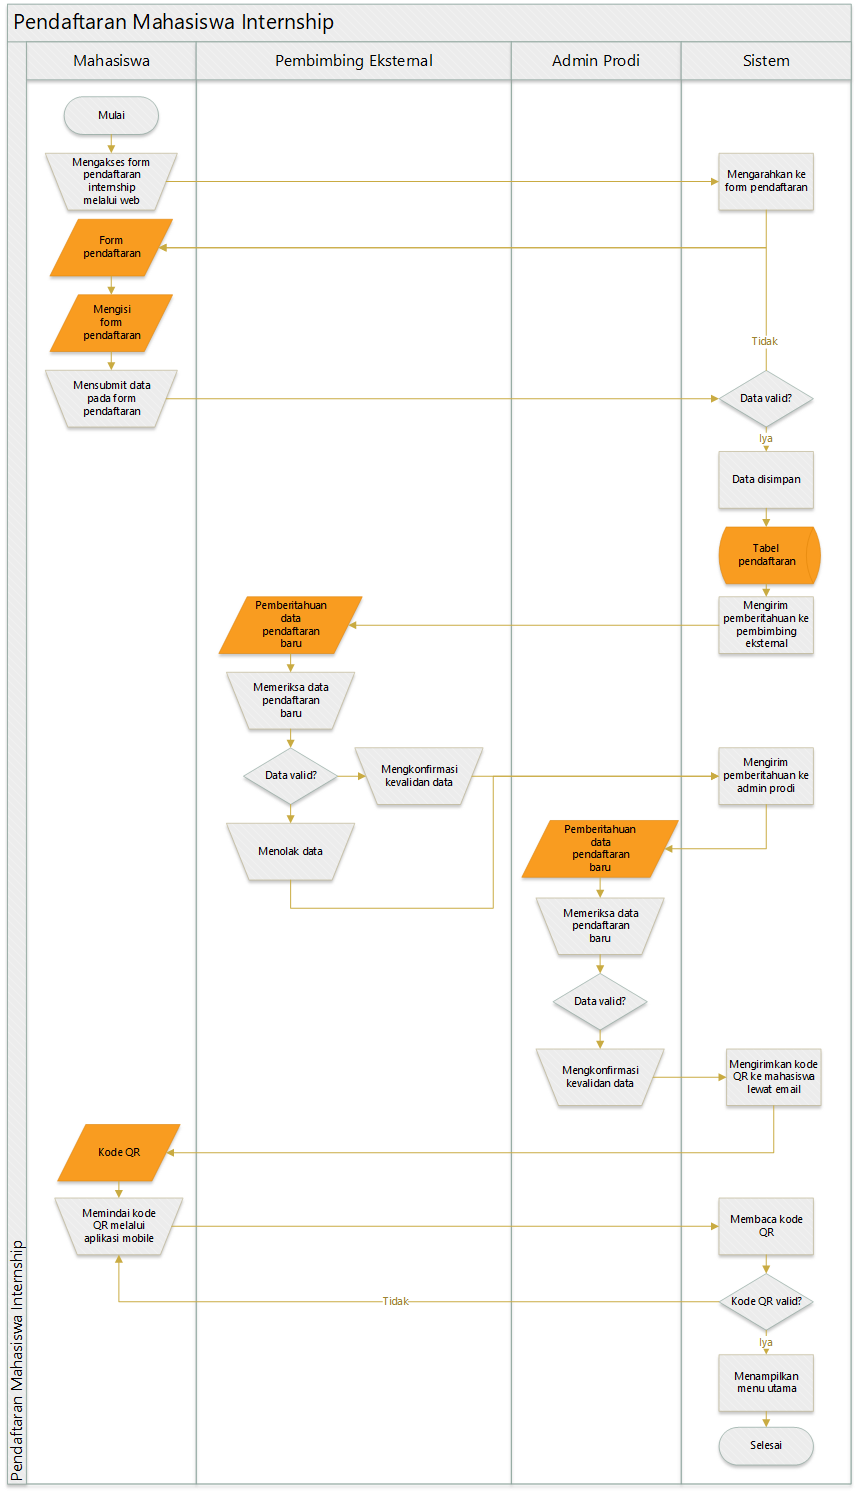
\includegraphics[width=10cm]{figures/image020.png}
		\centering
		\caption{Flowmap analisis yang akan dibangun pada pendaftaran mahasiswa internship }
	\end{figure}
\subsection{Analisis Sistem yang Akan Dibangun Pada Absensi Mahasiswa Internship}
Pada proses absensi mahasiswa melibatkan mahasiswa, pembimbing eksternal, pembimbing internal, dan admin prodi. Adapun mekanisme kerja yang dibuat adalah sebagai berikut:
\begin{enumerate}
	\item Mahasiswa membuka aplikasi mobile dan mengklik menu absensi.
	\item Mahasiswa mengisi data absensi di lokasi perusahaan internship dan mensubmit datanya
	\item Pembimbing eksternal memeriksa data absensi. Jika data benar maka akan dikonfirmasi
\end{enumerate}
	\begin{figure}[H]
		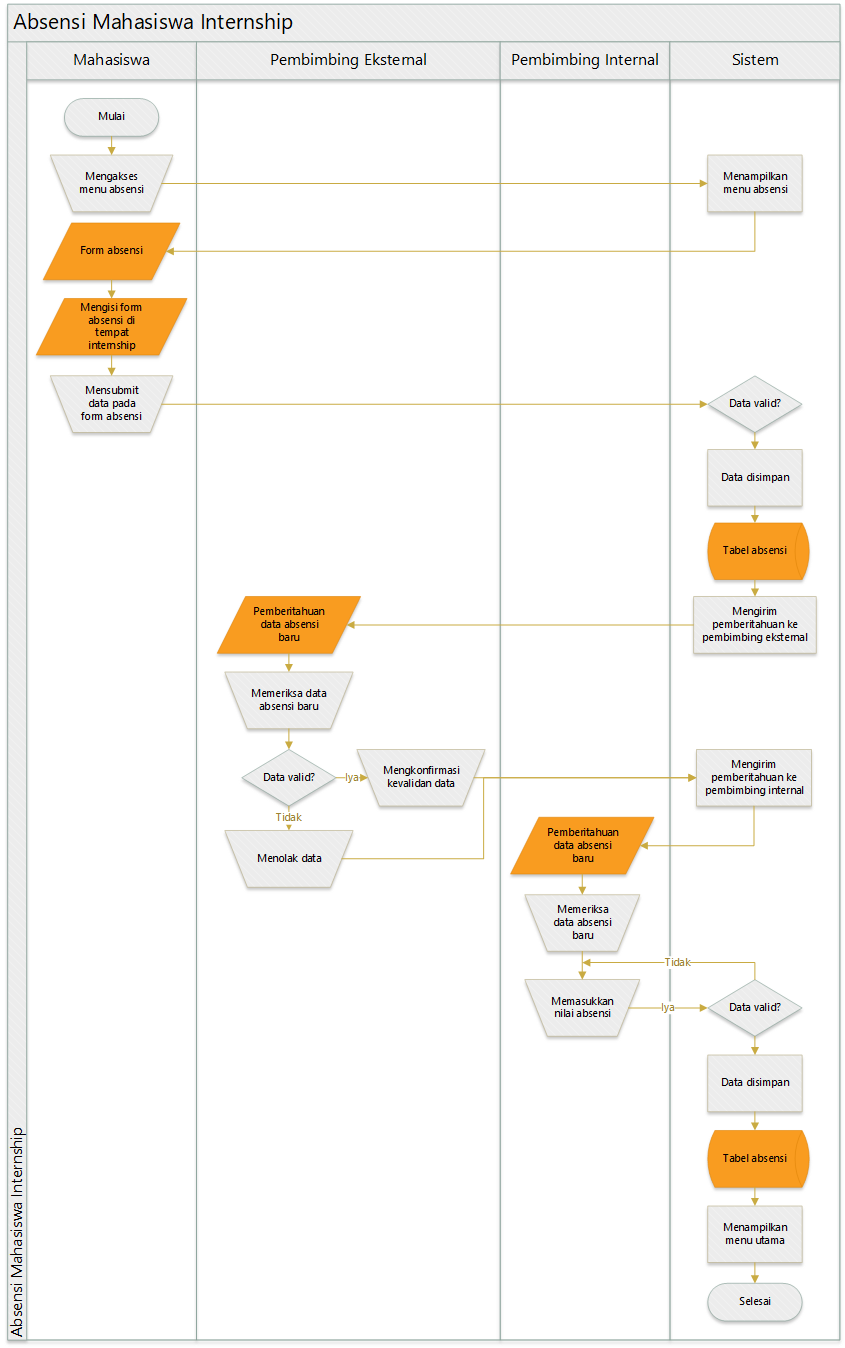
\includegraphics[width=10cm]{figures/image021.png}
		\centering
		\caption{Flowmap analisis yang akan dibangun pada absensi mahasiswa}
	\end{figure}
\subsection{Analisis Kebutuhan Fungsional}
Analisis kebutuhan fungsional merupakan suatu kebutuhan yang mencakup proses-proses yang berhubungan dengan kebutuhan sistem yang dibuat. Dimana menguraikan tentang fungsi-fungsi yang dapat membantu jalannya sistem. Adapun kebutuhan fungsional yang akan dibuat adalah sebagai berikut:
\begin{enumerate}
	\item Login User
	\item Registrasi User
	\item Pengelolaan data prodi
	\item Pengelolaan data dosen
	\item Pengelolaan data Internship
	\item Pengelolaan data mahasiswa
	\item Pengelolaan data absensi
	\item Pengelolaan data kegiatan
	\item Pengelolaan data user
	\item Ambil absensi
	\item Lihat progres absensi
\end{enumerate}
Setiap proses memiliki fungsi masing-masing pada sebuah tabel atau data yang terdapat pada database yang telah dirancang sebelumnya. Dan setiap proses berbubungan langsung dengan entitas atau user
\subsection{Analisis Kebutuhan Non Fungsional}
Analisis kebutuhan non fungsional dilakukan untuk mengetahui spesifikasi kebutuhan untuk perancangan sistem. Meliputi operasional sistem, dan keamanan sistem. Spesifikasi kebutuhan melibatkan analisis perangkat keras (hardware) dan perangkat lunak (software). Adapun kebutuhan non fungsional yang akan dibuat adalah sebagai berikut
\begin{itemize} 	
	\item Kebutuhan Perangkat Keras (Hardware) : Analisis tersebut digunakan untuk membantu proses pengolahan data, seperti input data, pemrosesan data dan output data
\begin{table}[h!]
\centering
\begin{tabular}{| l | l | p{3cm} | p{3cm} |} 
 \hline
 \textbf{No}   & \textbf{Nama Perangkat} & \textbf{Spesifikasi} &\textbf{Keterangan}\\ 
\hline
1   & Hardisk & 1 TB & Media untuk menyimpan data aplikasi yang dibuat. \\ 
\hline
2   & Memory & 4 GB & Memory system yang digunakan. \\ 
\hline
3   & Processor & AMD Ryzen 3 2200U 3.4 GHz & Untuk pemrosesan data \\ 
 \hline
\end{tabular}
\caption{Deskripsi Minimal Perangkat Keras Web Administrator}
\label{table:2}
\end{table}

\begin{table}[h!]
\centering
\begin{tabular}{| l | l | p{3cm} | p{3cm} |} 
 \hline
 \textbf{No}   & \textbf{Nama Perangkat} & \textbf{Spesifikasi} &\textbf{Keterangan}\\ 
\hline
1   & Hardisk & 32 TB & Tempat menyimpan data.. \\ 
\hline
2   & Memory & 3 GB & Kecepatan client dalam mengakses system ini.. \\ 
\hline
3   & Processir & Snapdragonn 439 & Untuk per-halamanisasi computer. \\ 
 \hline
4   & Kamera & 8MP & Untuk foto. \\ 
 \hline
\end{tabular}
\caption{Deskripsi Minimal Perangkat Keras Mobile}
\label{table:3}
\end{table}
	\item Kebutuhan Perangkat Lunak (Software) : Adapun spesifikasi perangkat lunak (software) yang dibutuhkan untuk mendukungaplikasi yang akan dibangun adalah sebagai berikut:
\begin{table}[h!]
\centering
\begin{tabular}{|c|c|c|} 
 \hline
 \textbf{No}   & \textbf{Tools} & \textbf{Fungsi}\\ 
\hline
1   & Windows 10 & Sistem operasi  \\ 
\hline
2   & XAMPP v2.3.3 & Web Server\\ 
\hline
3   & PHP Framework & Bahasa Pemrograman\\ 
 \hline
4   & Google Chrome& Web Browser  \\ 
 \hline
\end{tabular}
\caption{Deskripsi Minimal Perangkat Lunak Web Administrator}
\label{table:4}
\end{table}

\begin{table}[h!]
\centering
\begin{tabular}{|c|c|c|} 
 \hline
 \textbf{No}   & \textbf{Tools} & \textbf{Fungsi}\\ 
\hline
1   & Android Oreo & Sistem operasi  \\ 
 \hline
\end{tabular}
\caption{Deskripsi Minimal Perangkat Lunak Mobile}
\label{table:5}
\end{table}
\end{itemize}
\subsection{Perancangan Sistem}	
Berikut ini adalah suatu gambar analisa data pada Perancangan Sistem Aplikasi Sistem Monitoring Kinerja Mahasiswa Internship Prodi DIV Teknik Informatika Berbasis GPS menggunakan notasi UML (Unified Modeling Language).
\subsection{Use Case Diagram}
Use case diagram adalah gambaran semua aktor, usecase dan interaksi untuk mengenalkan suatu sistem. Dimana didalam usecase diagram menjelaskan tentang gambaran singkat hubungan antara actor dan usecase.
	\begin{figure}[H]
		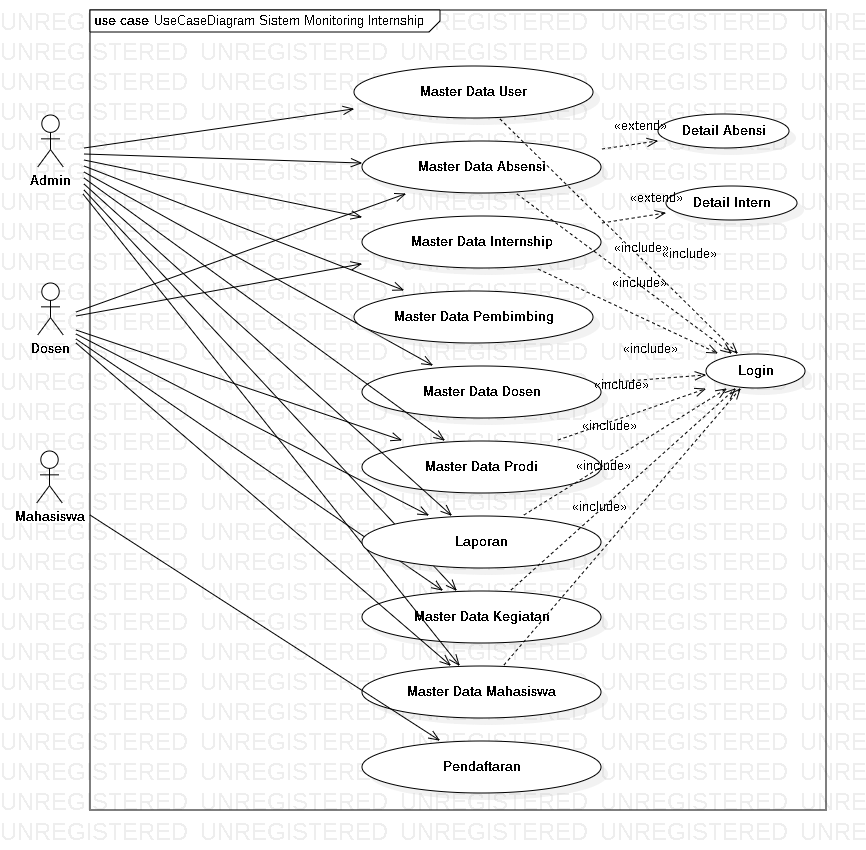
\includegraphics[width=10cm]{figures/diagram/image022.png}
		\centering
		\caption{Usecase Web }
	\end{figure}
	\begin{figure}[H]
		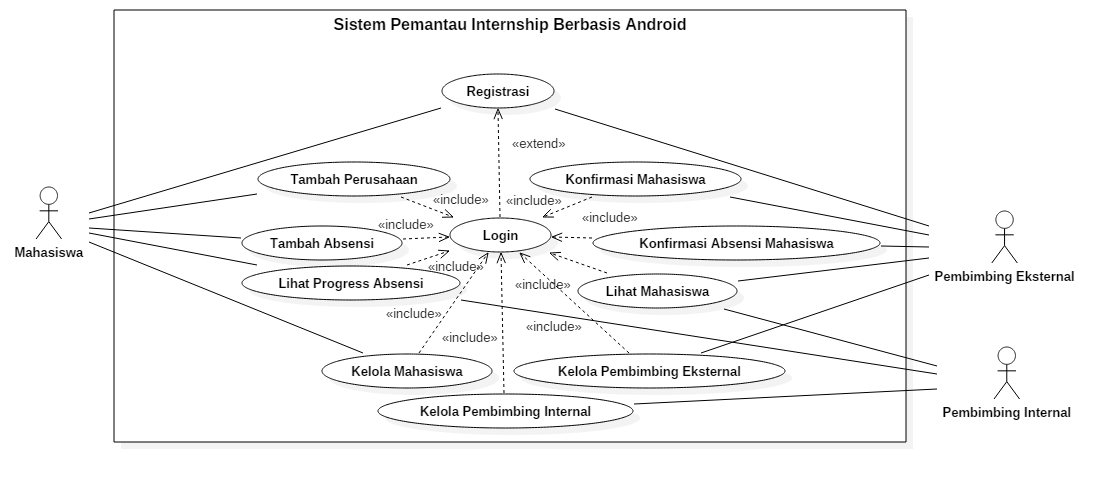
\includegraphics[width=10cm]{figures/diagram/image023.png}
		\centering
		\caption{Usecase Mobile }
	\end{figure}
\subsection{Definisi Aktor Web Administrator}
Pada bagian ini akan dijelaskan aktor-aktor yang terlibat.
\begin{table}[h!]
\centering
\begin{tabular}{| l | p{2cm} | p{9cm} |} 
 \hline
 \textbf{No}   & \textbf{Aktor} & \textbf{Deskripsi}\\ 
\hline
1   & Admin & Mengelola prodi,dosen,mahasiswa,internship,absensi,kegiatan,user\\ 
\hline
2   & Dosen & Mengelola profile,mahasiswa,absensi dan kegiatan  \\ 
\hline
3   & Mahasiswa & Melakukan registrasi \\  
 \hline
\end{tabular}
\caption{Aktor pada usecase web}
\label{table:6}
\end{table}
\subsection{Definisi Aktor Mobile Client}
Pada bagian ini akan dijelaskan aktor-aktor yang terlibat.

\begin{table}[h!]
\centering
\begin{tabular}{| l | p{3cm} | p{8cm} |} 
 \hline
 \textbf{No}   & \textbf{Aktor} & \textbf{Deskripsi}\\ 
\hline
1   & Mahasiswa & Melakukan registrasi, Melakukan tambah perusahaan, Melakukan tambah absens,i Melihat data progres absensi pribadi mahasiswa, Mengelola data pribadi mahasiswa\\ 
\hline
2   & Pembimbing Eksternal & Melakukan registrasi, Melakukan konfirmasi mahasiswa bimbingannya, Melakukan konfirmasi absensi mahasiswa bimbingannya ,Melihat data mahasiswa bimbingannya, Mengelola data pribadi pembimbing eksternal\\ 
\hline
3   & Pembimbing Internal & Melihat data mahasiswa bimbingannya,Melihat data progres absensi mahasiswa bimbingannya,Mengelola data pribadi pembimbing internal
 \\  
 \hline
\end{tabular}
\caption{Penjelasan Definisi Aktor Mobile Client}
\label{table:7}
\end{table}

\newpage

\subsection{Definisi Use Case Web Administrator }	
\begin{table}[h!]
\centering
\begin{tabular}{| l | p{5cm} | p{5cm} |} 
 \hline
 \textbf{No}   & \textbf{Aktor} & \textbf{Deskripsi}\\ 
\hline
1   & Login & Melakukan aktivitasi validasi pengguna ketika akan masuk\\ 
\hline
2   & Mengelola Prodi & Merupakan hak kelola prodi.\\ 
\hline
3   & Mengelola Dosen & Merupakan hak kelola Dosen.\\ 
 \hline
4   & Mengelola Mahasiswa & Merupakan hak kelola Mahasiswa.\\ 
 \hline
5   & Mengelola Internship & Merupakan hak kelola Internship.\\ 
 \hline
6   & Mengelola Absensi & Merupakan hak kelola Absensi.\\ 
 \hline
7   & Mengelola Kegiatan & Merupakan hak kelola Kegiatan.\\ 
 \hline
8   & Mengelola User & Merupakan hak kelola User.\\ 
 \hline
9   & Register & Merupakan proses membuat akun\\ 
 \hline
\end{tabular}
\caption{Penjelasan Definisi Use Case Web Administrator}
\label{table:8}
\end{table}

\newpage

\subsection{Definisi Use Case Mobile Client }	
\begin{table}[h!]
\centering
\begin{tabular}{| l | p{4cm} | p{6cm} |} 
 \hline
 \textbf{No}   & \textbf{Aktor} & \textbf{Deskripsi}\\ 
\hline
1   & Registrasi & Mahasiswa dan pembimbing bisa melakukan registrasi yang nantinya dapat masuk ke halaman sistem masing masing\\ 
\hline
2   & Login& Setiap user dapat login dan masuk ke halamannya masing masing.\\ 
\hline
3   & Tambah Perusahaan & Melakukan proses penambahan perusahaan tempat internship untuk mahasiswa.\\ 
 \hline
4   & Tambah Absensi & Melakukan proses penambahan absensi untuk mahasiswa.\\ 
 \hline
5   & Lihat Progres Absensi & Melihat progres absensi pribadi mahasiswa bagi  mahasiswa dan pembimbing Internal.\\ 
 \hline
6   & Kelola Mahasiswa & Melihat dan mengubah data mahasiswa.\\ 
 \hline
7   & Konfirmasi Mahasiwa & Proses konfirmasi mahasiswa untuk pembimbing eksternal.\\ 
 \hline
8   & Konfirmasi Absensi Mahasiswa & Proses konfirmasi absensi mahasiswa untuk pembimbing internal.\\ 
 \hline
9   & Lihat Mahasiswa & Melihat data mahasiswa bimbingannya untuk pembimbing eksternal dan internal\\ 
 \hline
10   & Kelola Pembimbing Eksternal & Melihat dan mengubah data pribadi pembimbing eksternal untuk pembimbing eksternal\\ 
 \hline
11  & Kelola Pembimbing Internal & Melihat dan mengubah data pribadi pembimbing internal untuk pembimbing internal\\ 
 \hline

\end{tabular}
\caption{Penjelasan Definisi Use Case Mobile Client}
\label{table:9}
\end{table}

\newpage
\subsection{Struktur Menu}
Adapun struktur menu yang digunakan adalah sebagai berikut.
\subsection{Struktur Menu Web}
	\begin{figure}[H]
		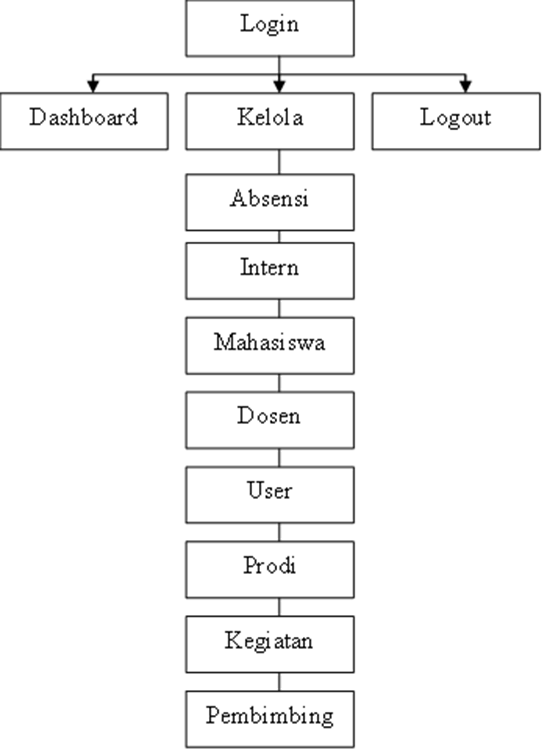
\includegraphics[width=6cm]{figures/diagram/image107.png}
		\centering
		\caption{Struktur Menu Admin }
	\end{figure}
		\begin{figure}[H]
		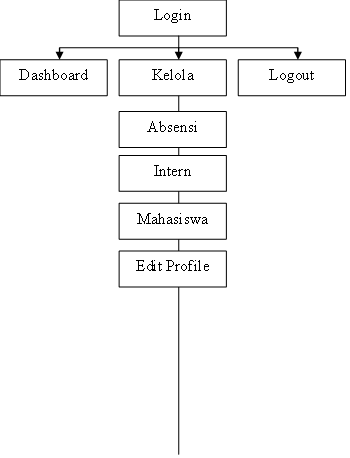
\includegraphics[width=6cm]{figures/diagram/image108.png}
		\centering
		\caption{Struktur Menu Dosen }
	\end{figure}

\subsection{Struktur Menu Mahasiswa Mobile Client}
	\begin{figure}[H]
		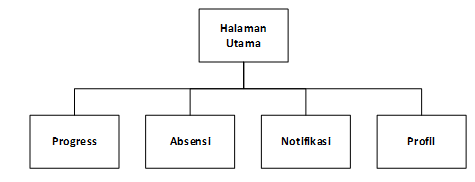
\includegraphics[width=6cm]{figures/diagram/image109.PNG}
		\centering
		\caption{Struktur Menu Mahasiswa Mobile Client }
	\end{figure}
	\begin{figure}[H]
		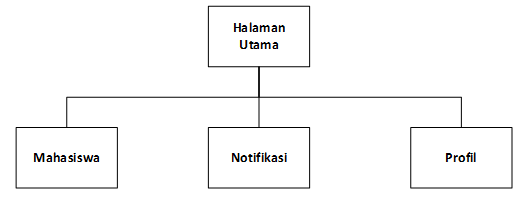
\includegraphics[width=6cm]{figures/diagram/image110.PNG}
		\centering
		\caption{Struktur Menu Pembimbing Internal Mobile Client }
	\end{figure}

\subsection{Struktur Menu Pembimbing Eksternal Mobile Client}
	\begin{figure}[H]
		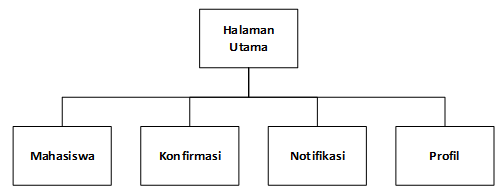
\includegraphics[width=6cm]{figures/diagram/image111.PNG}
		\centering
		\caption{Struktur Menu Pembimbing Internal Mobile Client }
	\end{figure}

\subsection{Perancangan Antarmuka}
\subsection{Perancangan Antarmuka Login Web}
	\begin{figure}[H]
		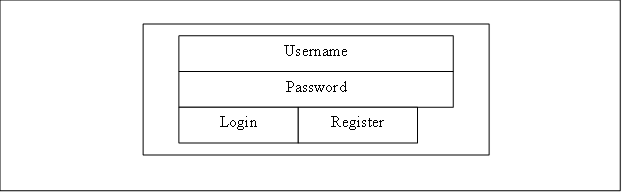
\includegraphics[width=6cm]{figures/diagram/image112.png}
		\centering
		\caption{Perancangan Antarmuka Halaman Login Web Administrator }
	\end{figure}
\subsection{Perancangan Antarmuka Dashboard Web Admin}
	\begin{figure}[H]
		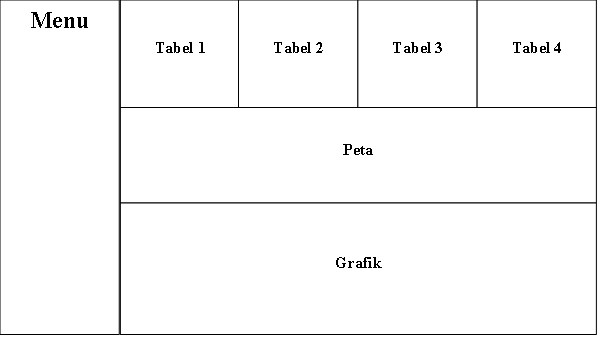
\includegraphics[width=6cm]{figures/diagram/image113.png}
		\centering
		\caption{Perancangan Antarmuka Halaman Dashboard Web Administrator}
	\end{figure}
\subsection{Perancangan Antarmuka Kelola Absensi Web Admin}
	\begin{figure}[H]
		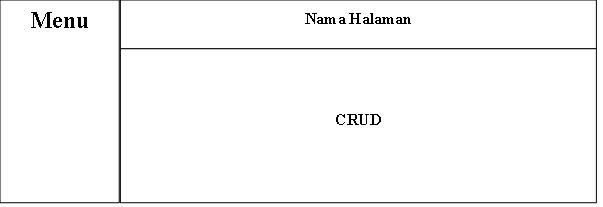
\includegraphics[width=6cm]{figures/diagram/image114.png}
		\centering
		\caption{Perancangan Antarmuka Halaman Kelola Absensi Web Administrator}
	\end{figure}
\subsection{Perancangan Antarmuka Kelola Internship Web Admin}
	\begin{figure}[H]
		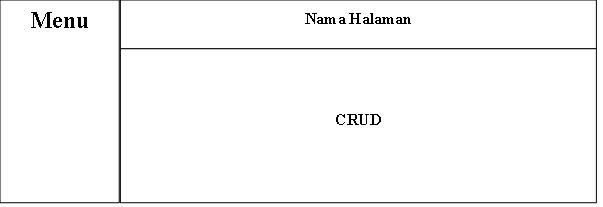
\includegraphics[width=6cm]{figures/diagram/image114.png}
		\centering
		\caption{Perancangan Antarmuka Halaman Kelola Internship Web Administrator}
	\end{figure}
\subsection{Perancangan Antarmuka Kelola Mahasiswa Web Admin}
	\begin{figure}[H]
		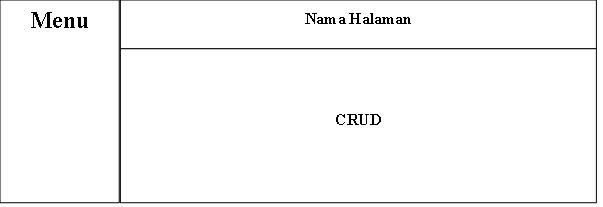
\includegraphics[width=6cm]{figures/diagram/image114.png}
		\centering
		\caption{Perancangan Antarmuka Halaman Kelola Mahasiswa Web Administrator}
	\end{figure}
\subsection{Perancangan Antarmuka Kelola Dosen Web Admin}
	\begin{figure}[H]
		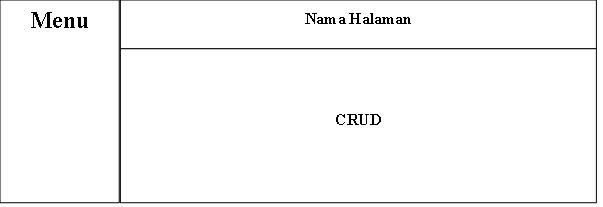
\includegraphics[width=6cm]{figures/diagram/image114.png}
		\centering
		\caption{Perancangan Antarmuka Halaman Kelola Dosen Web Administrator}
	\end{figure}
\subsection{Perancangan Antarmuka Kelola User Web Admin}
	\begin{figure}[H]
		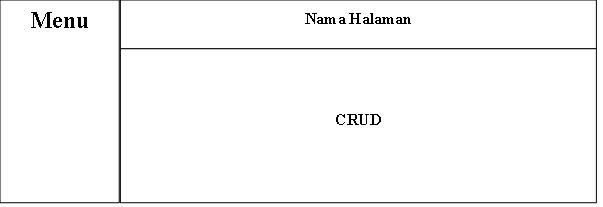
\includegraphics[width=6cm]{figures/diagram/image114.png}
		\centering
		\caption{Perancangan Antarmuka Halaman Kelola User Web Administrator}
	\end{figure}
\subsection{Perancangan Antarmuka Kelola Prodi  Web Admin}
	\begin{figure}[H]
		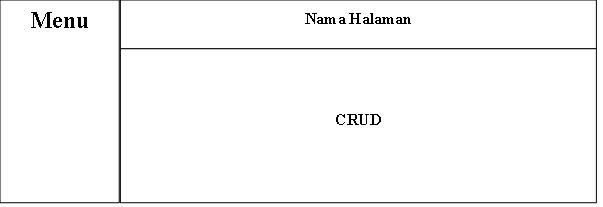
\includegraphics[width=6cm]{figures/diagram/image114.png}
		\centering
		\caption{Perancangan Antarmuka Halaman Kelola Prodi Web Administrator}
	\end{figure}
\subsection{Perancangan Antarmuka Kelola Kegiatan Web Admin}
	\begin{figure}[H]
		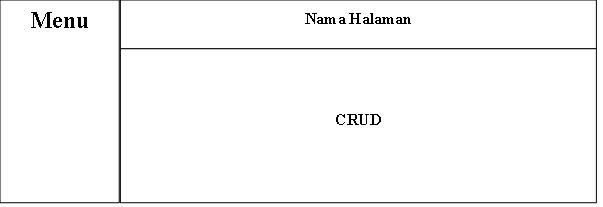
\includegraphics[width=6cm]{figures/diagram/image114.png}
		\centering
		\caption{Perancangan Antarmuka Halaman Kelola Kegiatan  Web Administrator}
	\end{figure}
\subsection{Perancangan Antarmuka Kelola Pembimbing  Web Admin}
	\begin{figure}[H]
		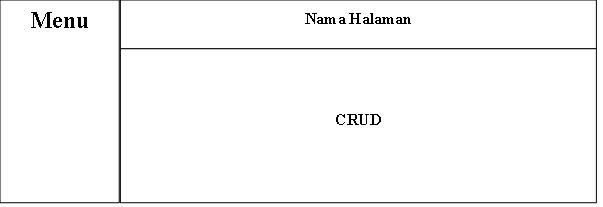
\includegraphics[width=6cm]{figures/diagram/image114.png}
		\centering
		\caption{Perancangan Antarmuka Halaman Kelola Pembimbing  Web Administrator}
	\end{figure}
\subsection{Perancangan Antarmuka Halaman Dashboard Web Dosen}
	\begin{figure}[H]
		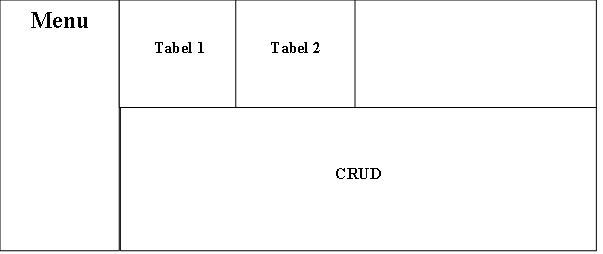
\includegraphics[width=6cm]{figures/diagram/image115.png}
		\centering
		\caption{Perancangan Antarmuka Halaman Dashboard Web Dosen}
	\end{figure}
\subsection{Perancangan Antarmuka Kelola Absensi Web Dosen}
	\begin{figure}[H]
		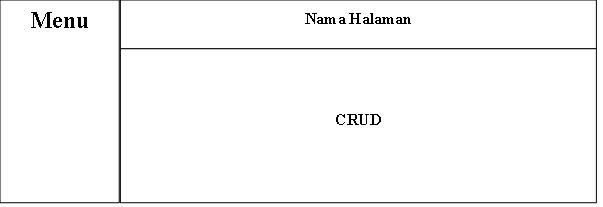
\includegraphics[width=6cm]{figures/diagram/image114.png}
		\centering
		\caption{Perancangan Antarmuka Halaman Kelola Absensi Web Dosen}
	\end{figure}
\subsection{Perancangan Antarmuka Kelola Internship Web Dosen}
	\begin{figure}[H]
		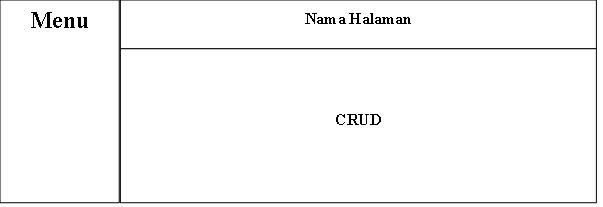
\includegraphics[width=6cm]{figures/diagram/image114.png}
		\centering
		\caption{Perancangan Antarmuka Halaman Kelola Internship Web Dosen}
	\end{figure}
\subsection{Perancangan Antarmuka View Mahasiswa Web Dosen}
	\begin{figure}[H]
		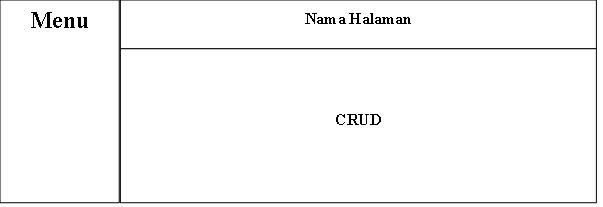
\includegraphics[width=6cm]{figures/diagram/image114.png}
		\centering
		\caption{Perancangan Antarmuka Halaman View Mahasiswa Web Dosen}
	\end{figure}
\subsection{Perancangan Antarmuka Kelola Profil Web Dosen}
	\begin{figure}[H]
		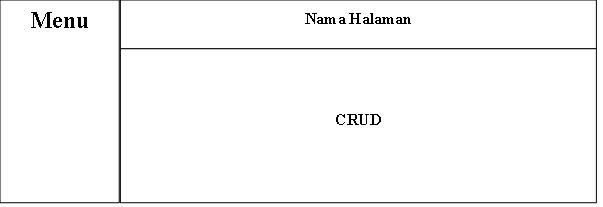
\includegraphics[width=6cm]{figures/diagram/image114.png}
		\centering
		\caption{Perancangan Antarmuka Halaman Kelola Profil  Web Dosen}
	\end{figure}
\subsection{Perancangan Antarmuka Registrasi Web }
	\begin{figure}[H]
		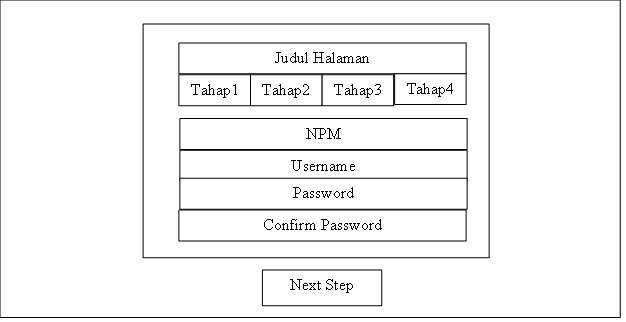
\includegraphics[width=6cm]{figures/diagram/image116.png}
		\centering
		\caption{Perancangan Antarmuka Halaman Registrasi 1}
	\end{figure}
	\begin{figure}[H]
		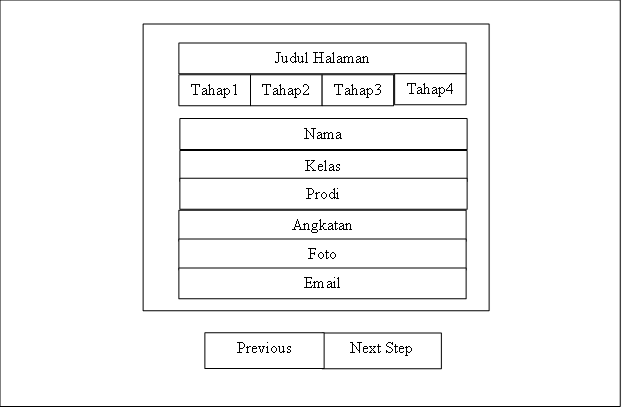
\includegraphics[width=6cm]{figures/diagram/image117.png}
		\centering
		\caption{Perancangan Antarmuka Halaman Registrasi 2}
	\end{figure}
	\begin{figure}[H]
		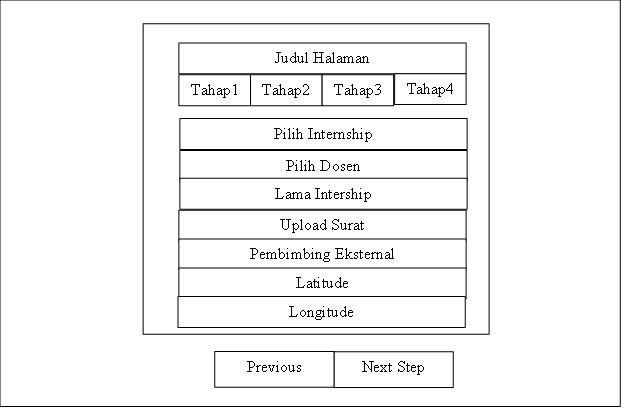
\includegraphics[width=6cm]{figures/diagram/image118.png}
		\centering
		\caption{Perancangan Antarmuka Halaman Registrasi 3}
	\end{figure}
	\begin{figure}[H]
		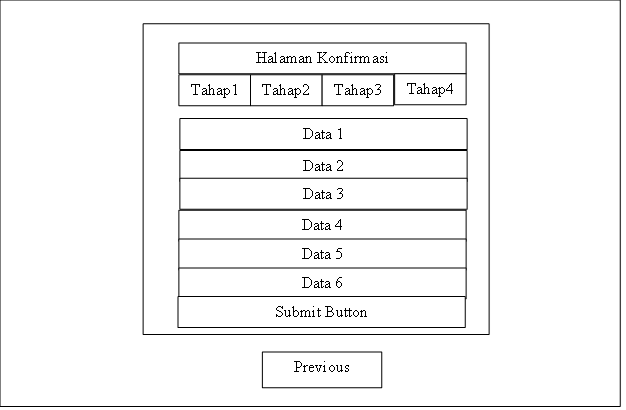
\includegraphics[width=6cm]{figures/diagram/image119.png}
		\centering
		\caption{Perancangan Antarmuka Halaman Registrasi 4}
	\end{figure}
\subsection{Perancangan Antarmuka Login Mobile Client }
	\begin{figure}[H]
		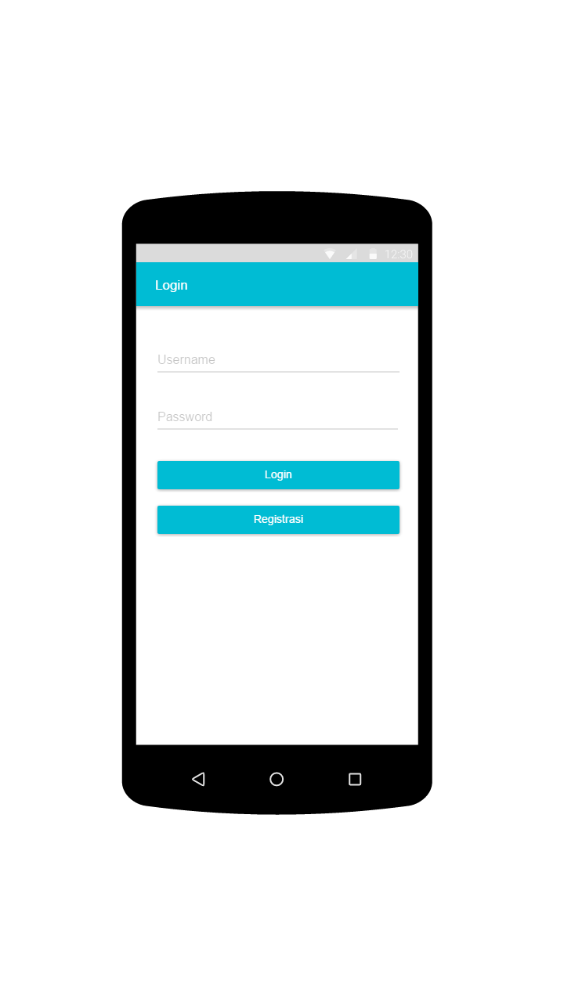
\includegraphics[width=6cm]{figures/diagram/image120.png}
		\centering
		\caption{Perancangan Antarmuka Login Mobile Client}
	\end{figure}
\subsection{Perancangan Antarmuka Registrasi Mahasiswa Mobile Client }
	\begin{figure}[H]
		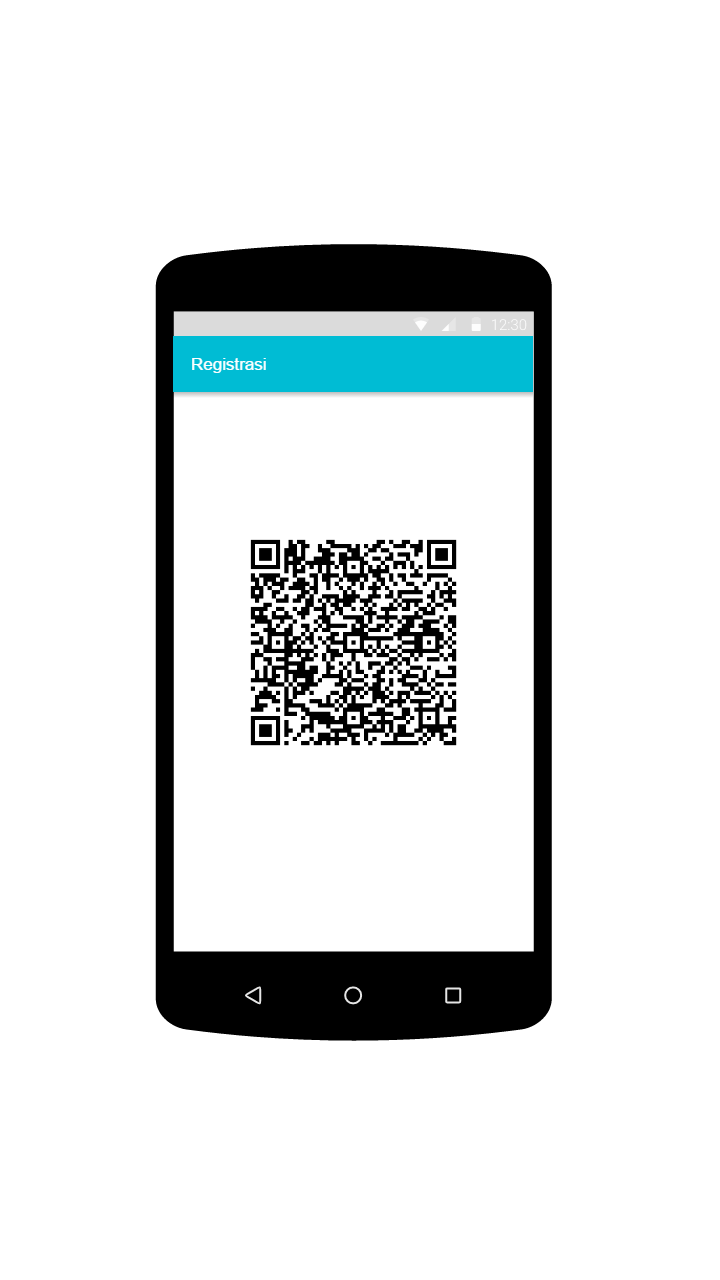
\includegraphics[width=6cm]{figures/diagram/image121.png}
		\centering
		\caption{Perancangan Antarmuka Registrasi Mahasiswa Mobile Client}
	\end{figure}
\subsection{Perancangan Antarmuka Tambah Perusahaan Mobile Client }
	\begin{figure}[H]
		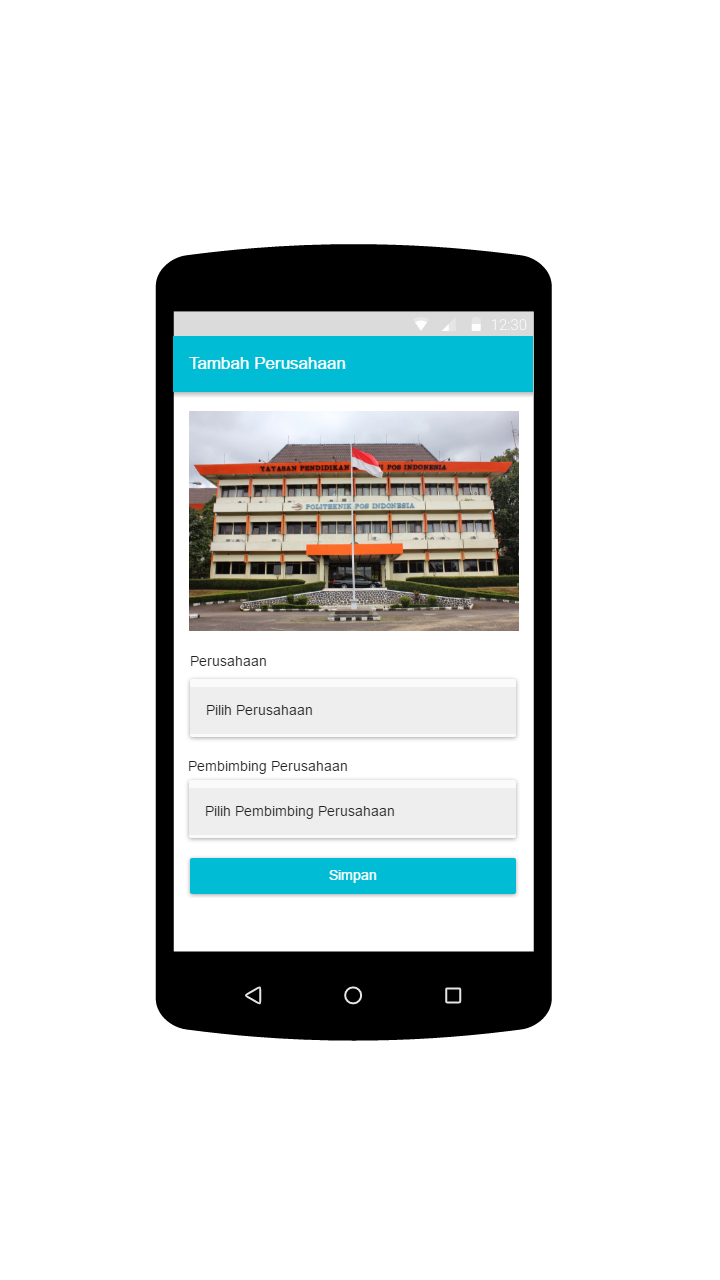
\includegraphics[width=6cm]{figures/diagram/image122.png}
		\centering
		\caption{Perancangan Antarmuka Tambah Perusahaan Mobile Client}
	\end{figure}
\subsection{Perancangan Antarmuka Progres Mahasiswa Mobile Client }
	\begin{figure}[H]
		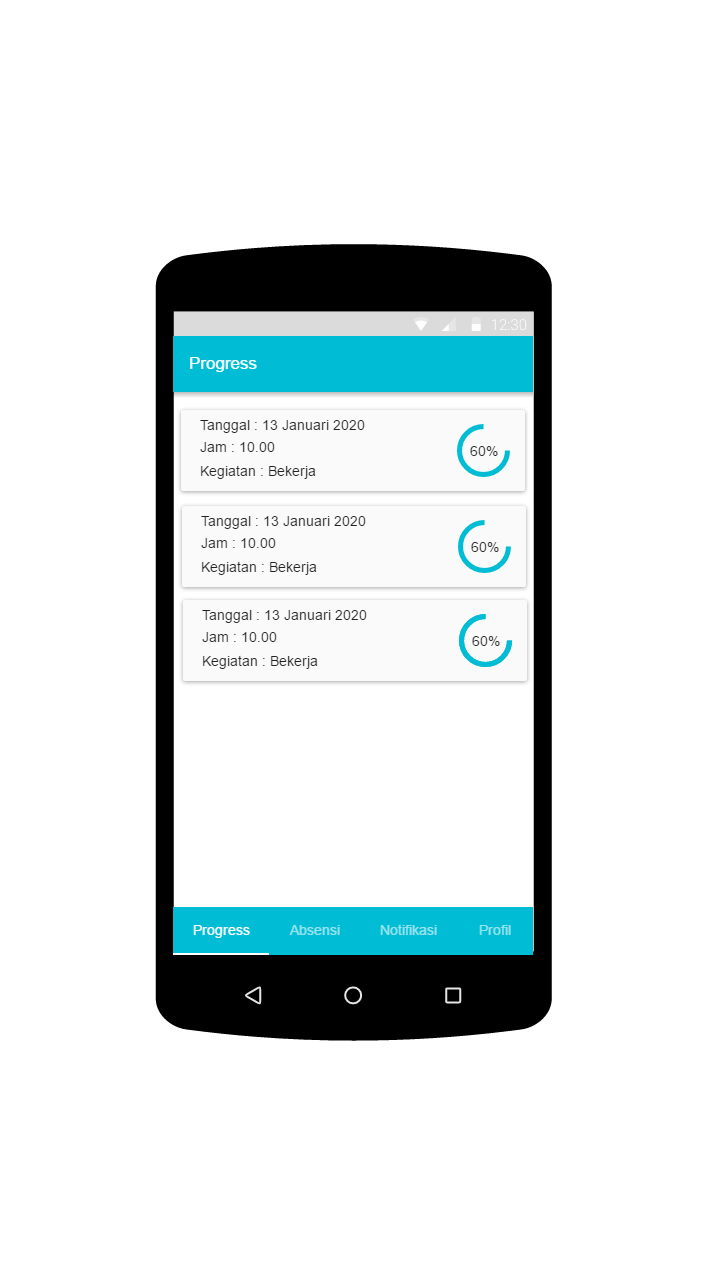
\includegraphics[width=6cm]{figures/diagram/image123.png}
		\centering
		\caption{Perancangan Antarmuka Progres Mahasiswa Mobile Client}
	\end{figure}
\subsection{Perancangan Antarmuka Absensi Mobile Client }
	\begin{figure}[H]
		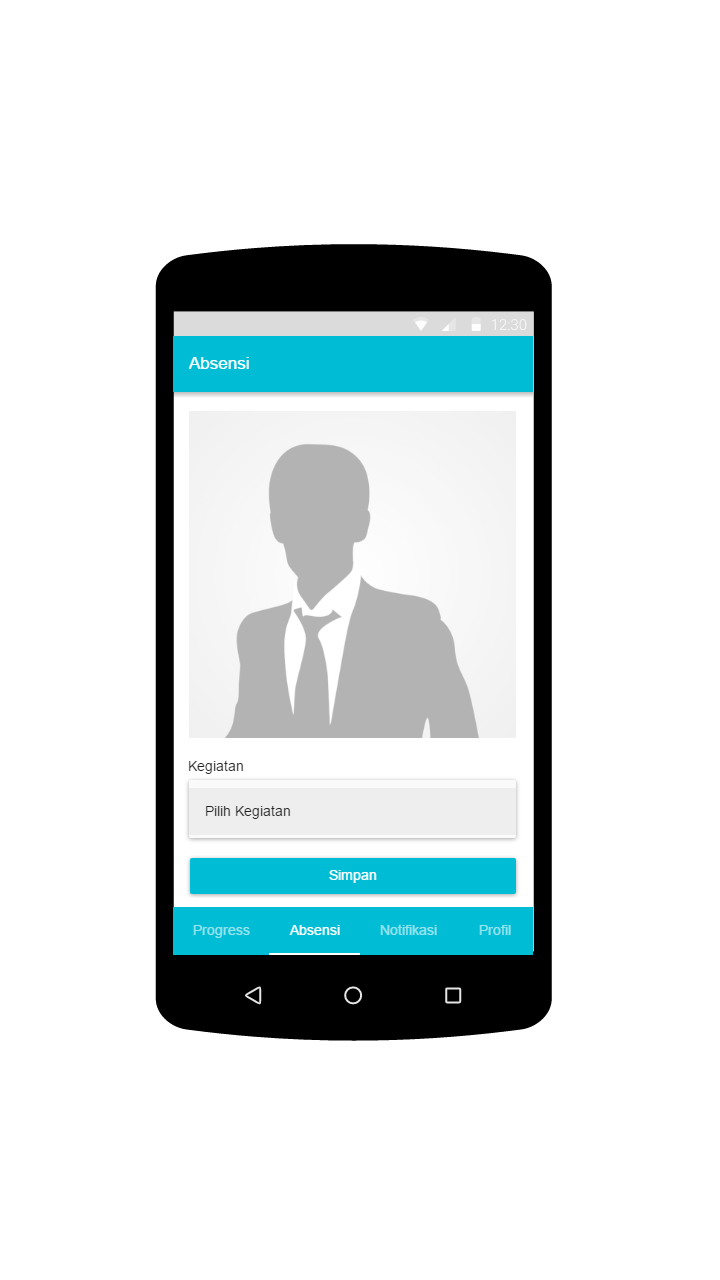
\includegraphics[width=6cm]{figures/diagram/image124.png}
		\centering
		\caption{Perancangan Antarmuka Absensi Mobile Client}
	\end{figure}
\subsection{Perancangan Antarmuka Notifikasi Mahasiswa  Mobile Client }
	\begin{figure}[H]
		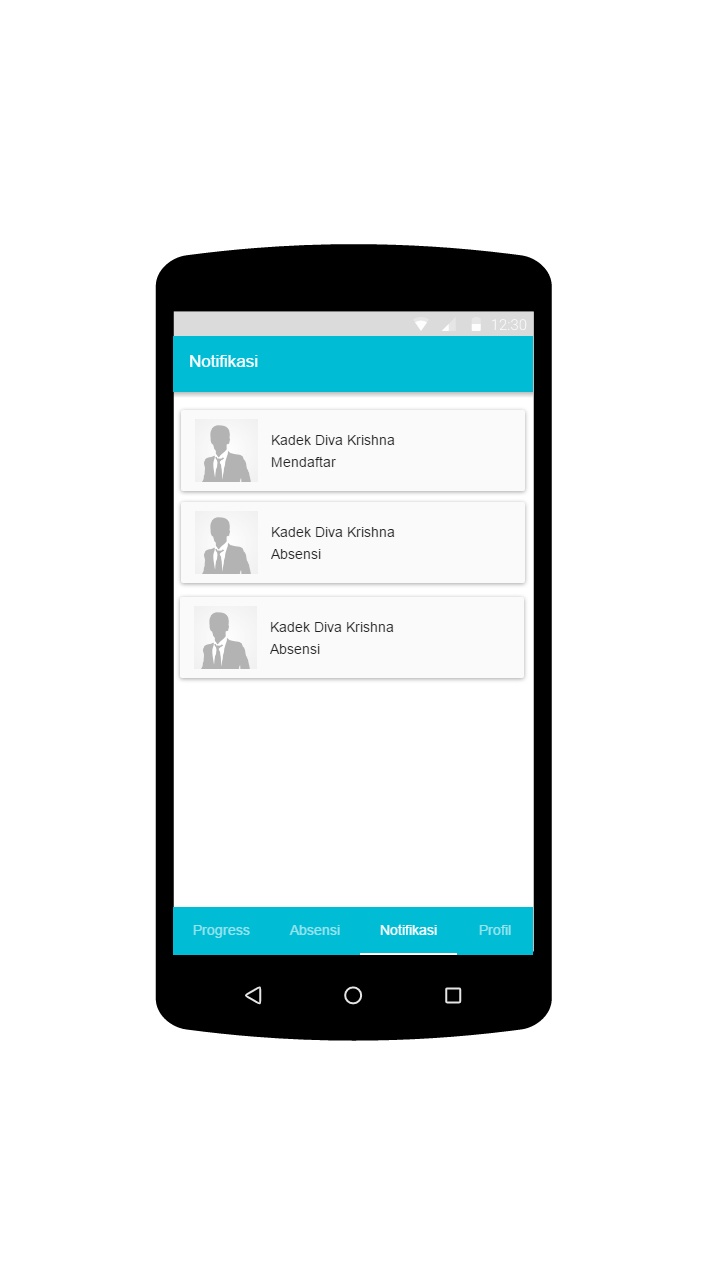
\includegraphics[width=6cm]{figures/diagram/image125.png}
		\centering
		\caption{Perancangan Antarmuka Notifikasi Mahasiswa  Mobile Client}
	\end{figure}
\subsection{Perancangan Antarmuka Profil Mahasiswa Mobile Client }
	\begin{figure}[H]
		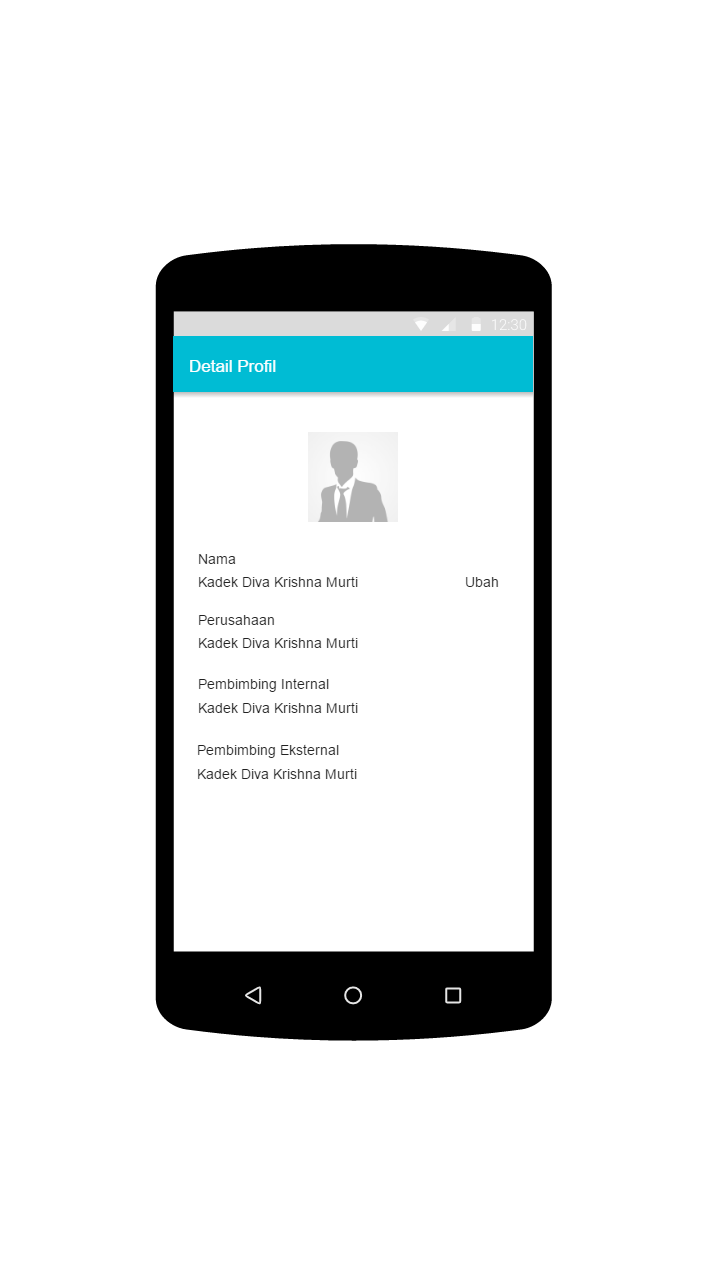
\includegraphics[width=6cm]{figures/diagram/image126.png}
		\centering
		\caption{Perancangan Antarmuka Profil Mahasiswa Mobile Client}
	\end{figure}
\subsection{Perancangan Antarmuka Ubah Password  Mobile Client }
	\begin{figure}[H]
		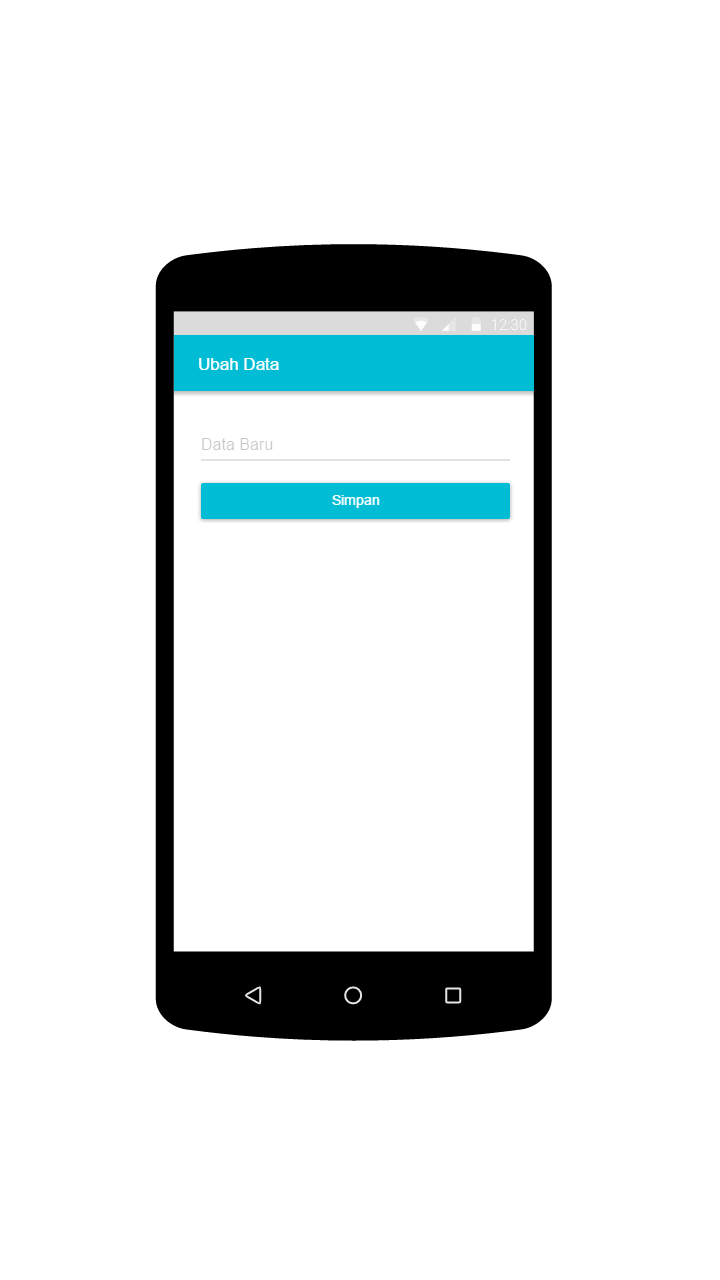
\includegraphics[width=6cm]{figures/diagram/image127.png}
		\centering
		\caption{Perancangan Antarmuka Ubah Password Mobile Client}
	\end{figure}
\subsection{Perancangan Antarmuka Registrasi Pembimbing Eksternal  Mobile Client }
	\begin{figure}[H]
		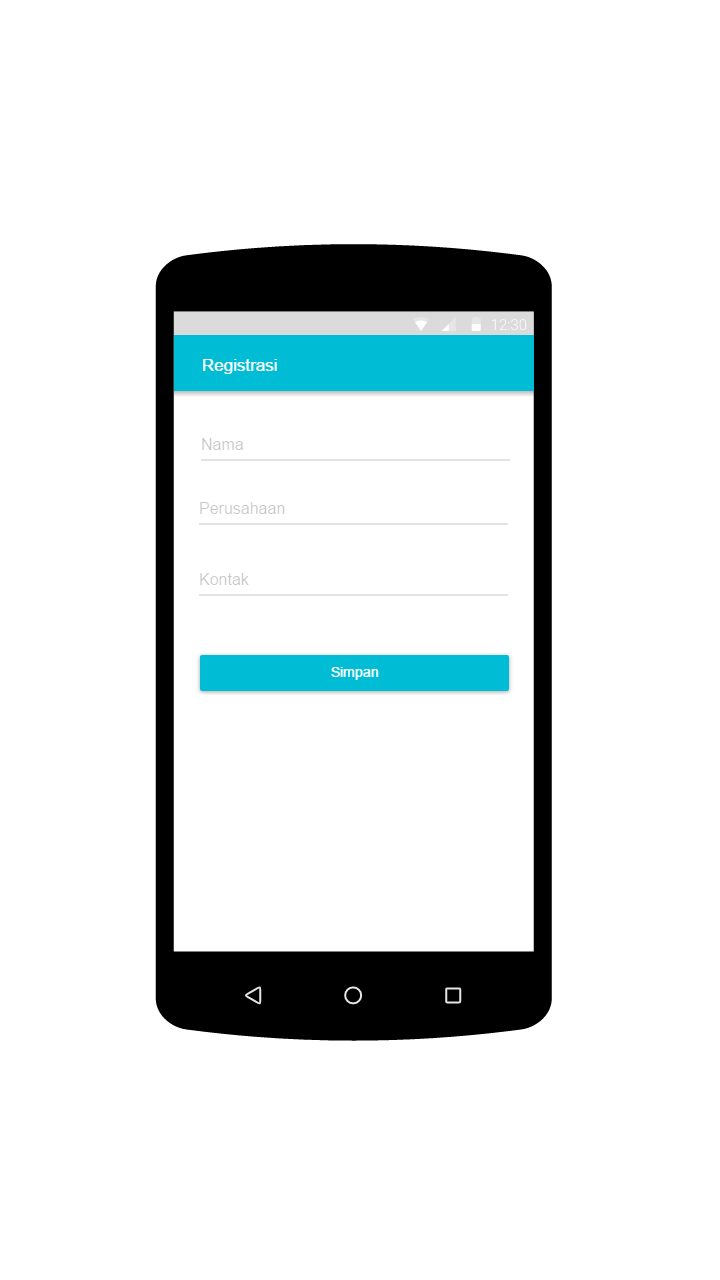
\includegraphics[width=6cm]{figures/diagram/image128.png}
		\centering
		\caption{Perancangan Antarmuka Registrasi Pembimbing Eksternal Mobile Client}
	\end{figure}
\subsection{Perancangan Antarmuka Data Mahasiswa Mobile Client }
	\begin{figure}[H]
		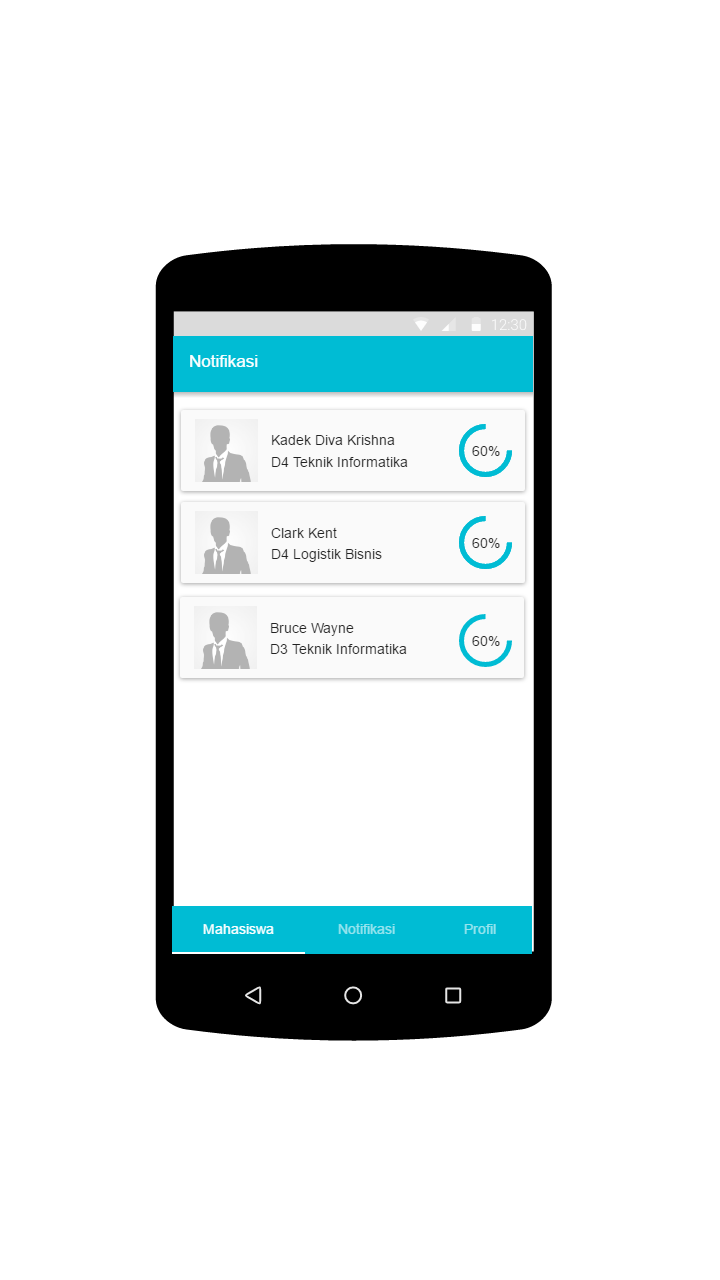
\includegraphics[width=6cm]{figures/diagram/image129.png}
		\centering
		\caption{Perancangan Antarmuka Data Mahasiswa Mobile Client}
	\end{figure}
\subsection{Perancangan Antarmuka Detail Mahasiswa Mobile Client }
	\begin{figure}[H]
		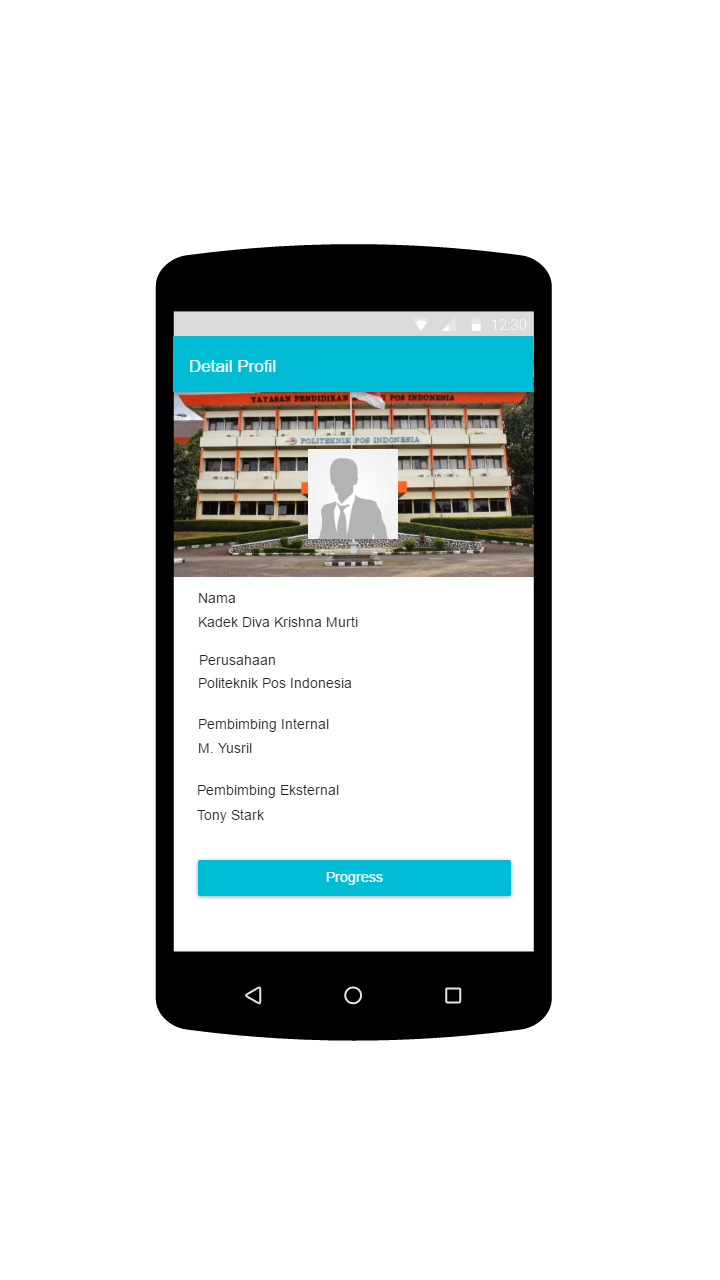
\includegraphics[width=6cm]{figures/diagram/image130.png}
		\centering
		\caption{Perancangan Antarmuka Detail Mahasiswa Mobile Client}
	\end{figure}
\subsection{Perancangan Antarmuka Progres Detail Mahasiswa Mobile Client }
	\begin{figure}[H]
		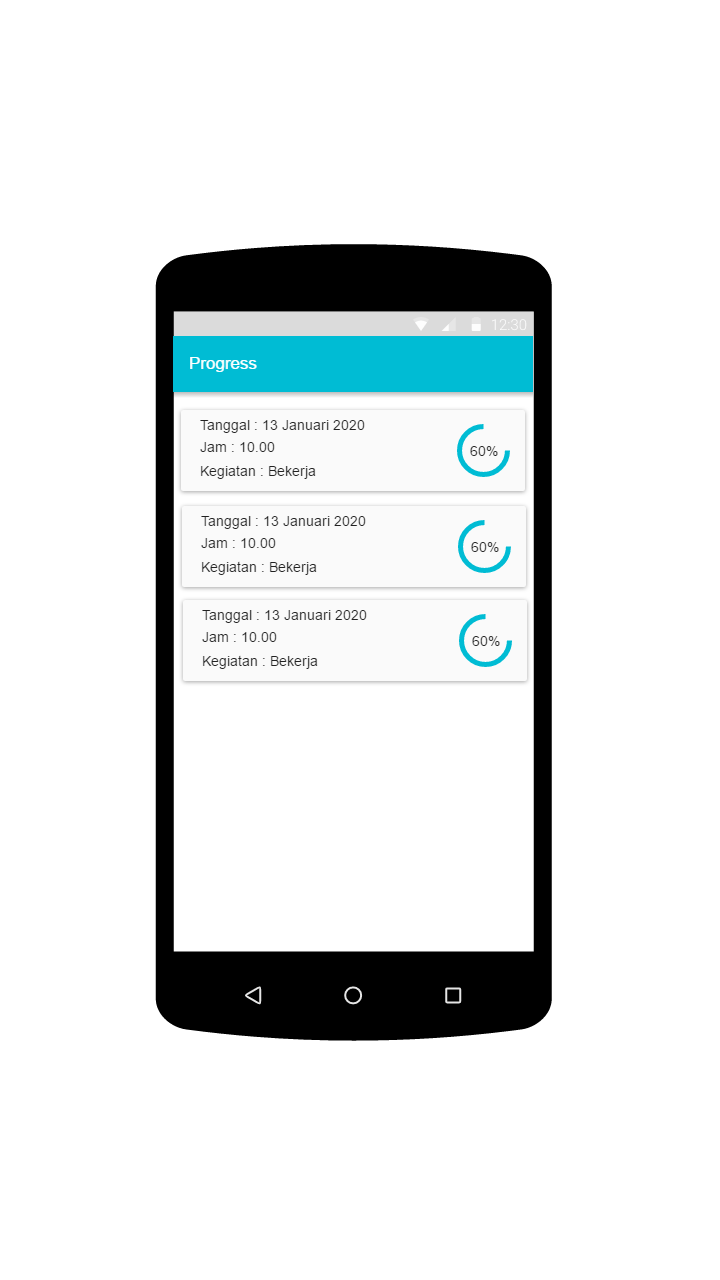
\includegraphics[width=6cm]{figures/diagram/image131.png}
		\centering
		\caption{Perancangan Antarmuka Progres Detail Mahasiswa Mobile Client}
	\end{figure}
\subsection{Perancangan Antarmuka Notifikasi Pembimbing Eksternal Mobile Client }
	\begin{figure}[H]
		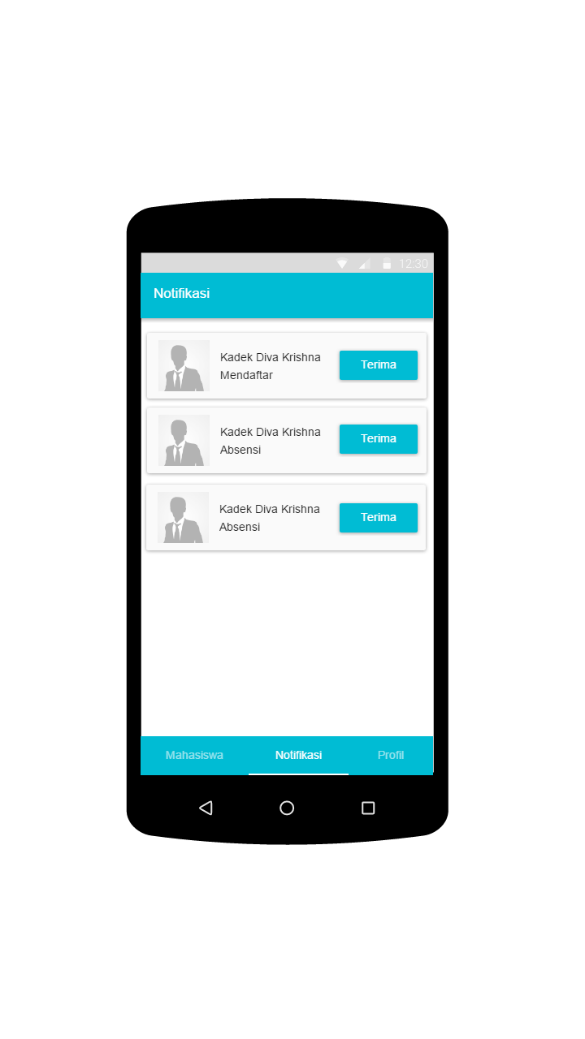
\includegraphics[width=6cm]{figures/diagram/image132.png}
		\centering
		\caption{Perancangan Antarmuka Notifikasi Pembimbing Eksternal Mobile Client}
	\end{figure}
\subsection{Perancangan Antarmuka Profil Pembimbing Internal dan Eksternal Mobile Client }
	\begin{figure}[H]
		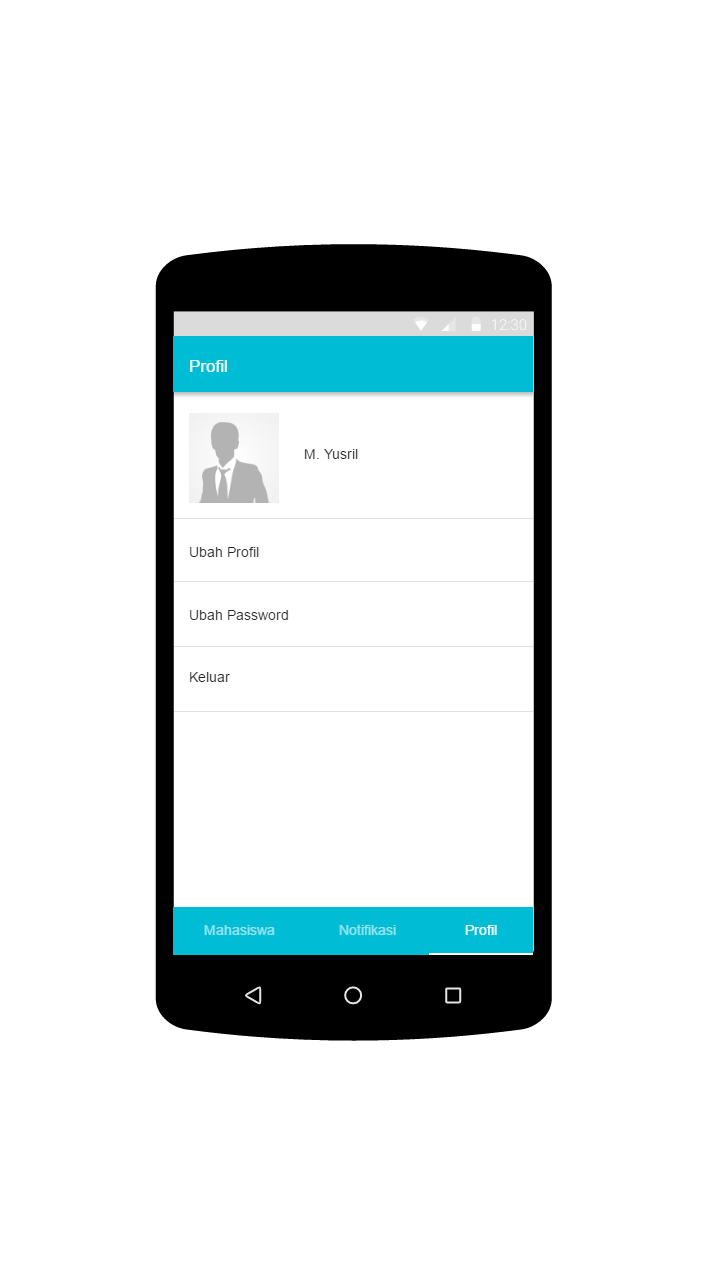
\includegraphics[width=6cm]{figures/diagram/image133.png}
		\centering
		\caption{Perancangan Antarmuka Profil Pembimbing Internal dan  Eksternal Mobile Client}
	\end{figure} 
\subsection{Perancangan Antarmuka Notifikasi Pembimbing Internal Mobile Client }
	\begin{figure}[H]
		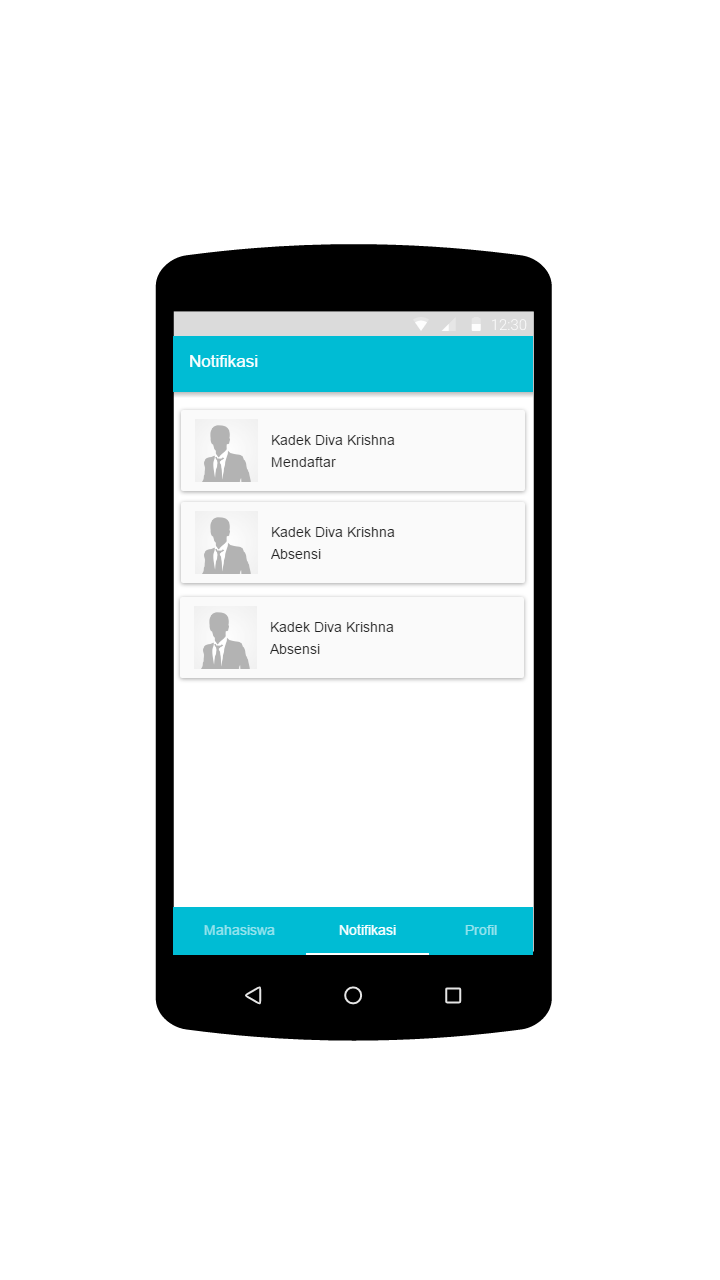
\includegraphics[width=6cm]{figures/diagram/image134.png}
		\centering
		\caption{Perancangan Antarmuka Notifikasi Pembimbing Internal Mobile Client}
	\end{figure} 